This thesis set out to design a software solution that uses the parametric L-system to representing complex plant-like structures, and to explore whether the L-system can provide the relavant information necessary for physical simulation. This chapter will show several features of the parametric L-system, such as how varying parameters like branch width and branching angles can affect the resulting visual effect on the plant models. Furthermore, parameters that manipulate the physical behaviour of the plant under forces like wind or gravity will be tested and their results will be discussed. All of the tests within this chapter are run on the same interpreter and physics simulation, with the acceleration due to gravity being kept at a constant value of $9.8m/s^2$. 

L-system \ref{parametric L-system results} defined below has a several parameters that affect the look and behaviour of the resulting plant. The parameters have been chosen as they each affect a perceptible property of plant when rendered or simulated.

The table below shows three sets of default values that will be applied to the L-system in each example. These parameters are numeric values and can be provided to the L-system by means of the \#define statements. For each test only one or two of these parameters will be manipulated and screenshots will show its affect on the structure or how it reacts in the physical simulation. These features have the the following meanings: 

\begin{itemize}[noitemsep]
	\item n - The number of generations to rewrite
	\item a1 - The angle of the first pitch rotation in production rule 1
	\item a2 - The angle of the second pitch rotation in production rule 1
	\item a3 - The angle of both roll rotations in production rule 1
	\item dl - The proportion to increase the branch length each generation
	\item dr - The proportion to increase the branch width each generation
	\item scstart - The starting spring constant 
	\item scmod - The proportion to increase the spring constant each generation
\end{itemize}

\begin{singlespace}
\begin{equation}
\begin{aligned}
	&\textrm{\#object F BRANCH;}\\
	&\textrm{\#w : !(1.4)F(2.0, scstart)/(45)A(scstart);}\\
	&\textrm{\#p1 : A(sc) : * : !(dr)F(2, sc)[\&(a3)F(2, sc)A(sc)]/(a1)[\&(a3)F(2, sc)A(sc)]/(a2)[\&(a3)F(2, sc)A(sc)];}\\
	&\textrm{\#p2 : F(l, sc) : * : F(l*dl, sc*scmod);}\\
	&\textrm{\#p3 : !(w) : * : !(w*dr);}
\end{aligned}
\end{equation} \label{parametric L-system results}
\end{singlespace}

\vspace{10mm}
\hrule
\begin{table}[h!]
\centering
\begin{tabular}{ | c | c | c | c | c | c | c | c | c | }
\hline
	Variation Name & n & a1 & a2 & a3 & dl & dr & scstart & scmod\\  
\hline
\hline
	L-system 1  & 6 & 112.5 & 157.5 & 22.5 & 1.1 & 1.4 & 200 & 1.0 \\
\hline
	L-system 2  & 6 & 137.5 & 137.5 & 18.95 & 1.1 & 1.2 & 200 & 1.0 \\
\hline
	L-system 3  & 7 & 112.5 & 157.5 & 22.5 & 1.1 & 1.4 & 200 & 1.0 \\
\hline
\end{tabular}
\caption{Table of turtle graphics instructions symbols and their meaning to the interpreter}
\label{L-system params}
\end{table}
\FloatBarrier
\hrule

\vspace{10mm} 

\noindent
In the example in figure \ref{example thickness}, the value `dr', manipulates how thick each branch is. It does this during the rewriting process. Every time the width module `!' is encountered, it is rewritten with the current radius multiplied by the value of `dr', which increases the radius exponentially. This relationship can be expressed as $r_{i+1} = r_i \times dr$, where $r_i$ is the current branch radius and $r_{i+1}$ is the radius of the branch in the next generation. This gives a tree that gets thicker exponentially as the branch moves closer to the base of the tree, as these branch instructions will be rewritten a greater number of times than the branch instructions near the top of three. This can be shown in the graphs in figure \ref{graph thickness} below. For a tree that gets thicker linearly, the relationship can be changed and expressed as $r_{i+1} = r_i + dr$. This would result in a tree that gets thicker much more progressively.

Although this example is not a physical simulation, it could be simulated. Due to the larger width of the branches near the base of the tree, they would have a higher mass and therefore have more inertia, making them more resistant to changes in velocity.

\begin{figure}[htbp]
	{\centering
		\vspace{7px}
		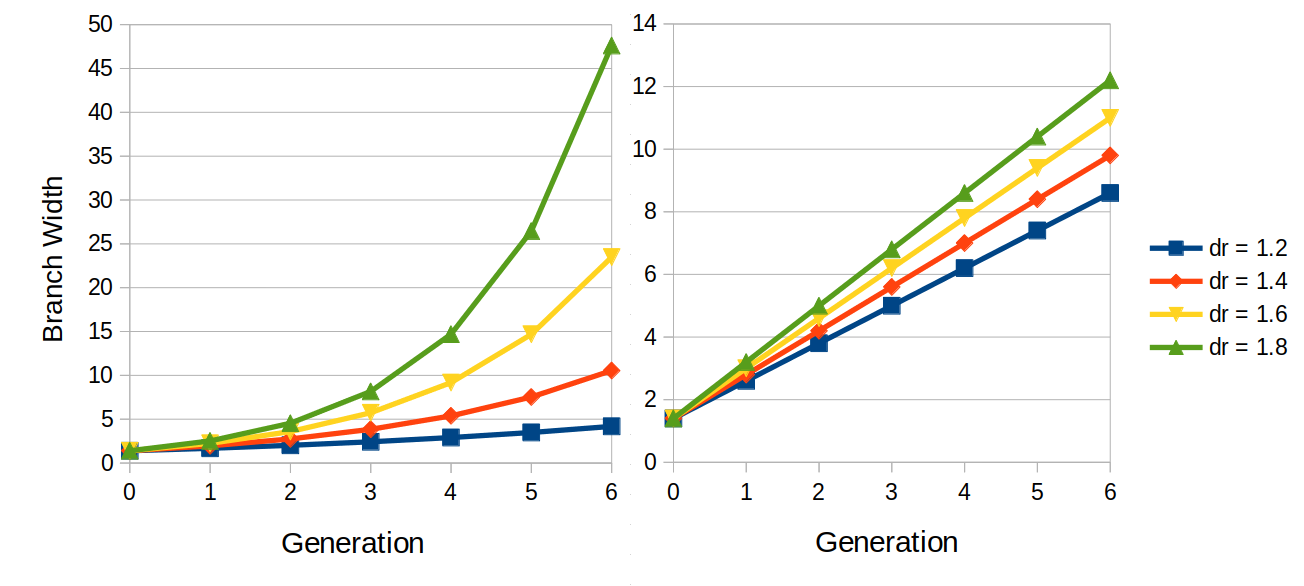
\includegraphics[scale=0.35]{Diagrams/branchWidthIncrease.png}
		\caption{Graph showing an exponential and linear relationship between the branch width and the generation when increasing the value of `dr'.} \label{graph thickness}
	}
\end{figure}
\FloatBarrier

\begin{figure}[htbp]
	{\centering
		\vspace{7px}
		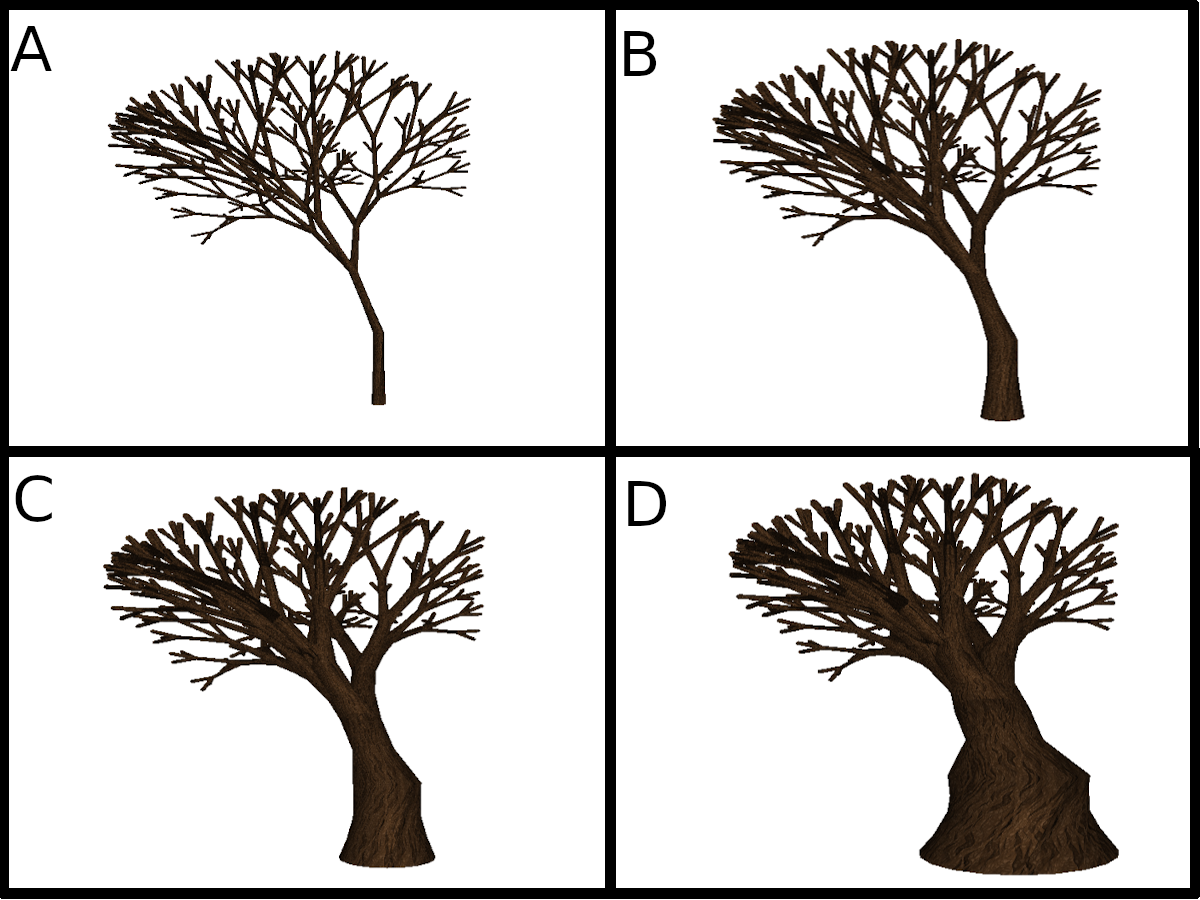
\includegraphics[scale=0.30]{Diagrams/TernaryBranching3_vr.png} 
		\caption{Examples of L-system 1 changing the `dr' variable which modifies the thickness of the base of the tree.} \label{example thickness}
	}
\end{figure}
\FloatBarrier

\noindent
Figure \ref{example angle} below shows that the result of changing the roll rotations' angle for some of the branches gives the tree a very different shape. In this case, increasing the angle of the branches' roll rotations from 15$^\circ$ to 30$^\circ$ can create a branch that curls slightly. Increasing this angle causes the result to be more dramatic. Furthermore, the angles of rotations can be randomised using the random range feature to have the same L-system produce many variations of the same structure. Manipulating the angles of rotations is a very powerful tool to allow very drastic changes to the look or behavior of a plant without changing its structure. 

\begin{figure}[htbp]
	{\centering
		\vspace{7px}
		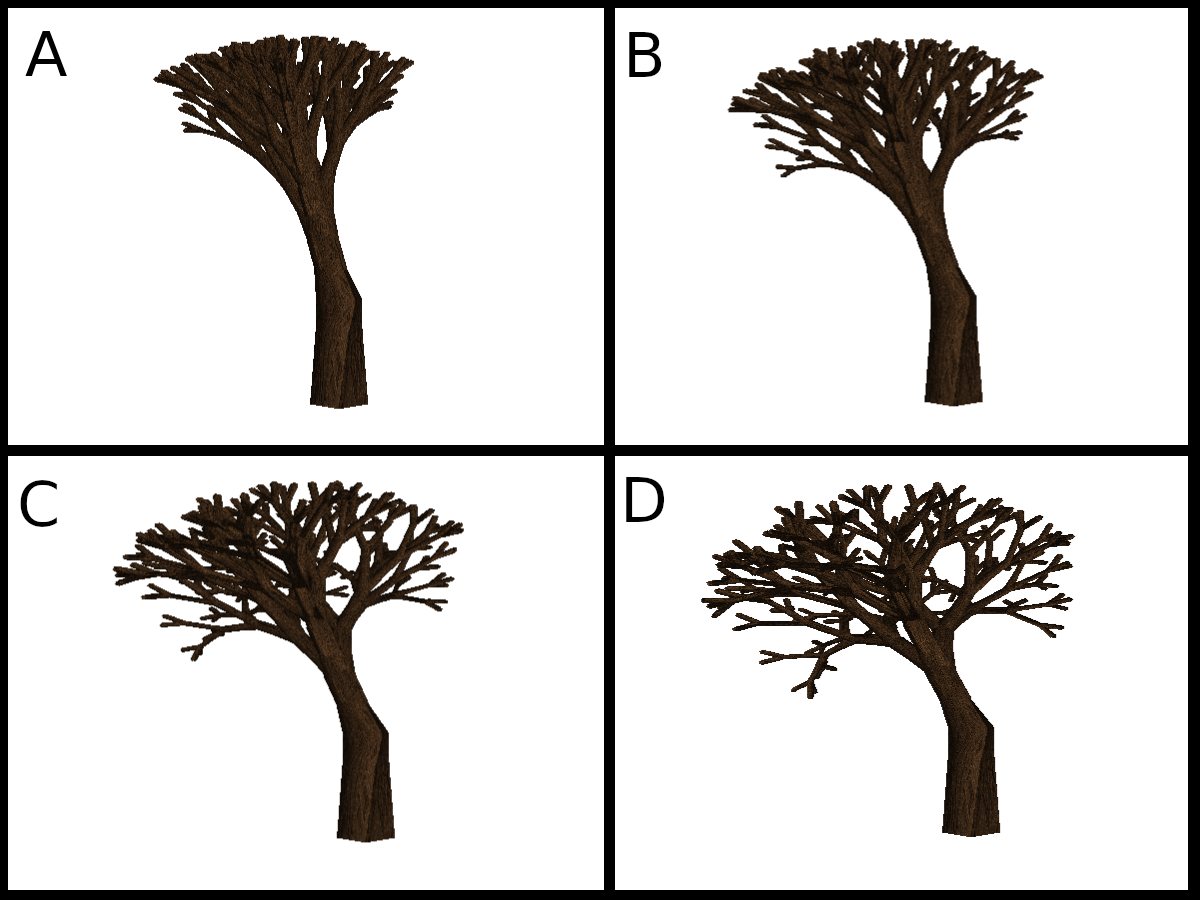
\includegraphics[scale=0.30]{Diagrams/TernaryBranching2_angle_example.png}
		\caption{Examples of L-system 2 changing the `a3' variable modifying the roll angle of certain branches.} \label{example angle}
	}
\end{figure}
\FloatBarrier

\noindent
If the angle is changed to 60$^\circ$ the tree looks almost unrecognisable to its original structure. This can be seen in figure \ref{extreme example angle} below. In this example the branches are rendered as green spheres in order to indicate that they are the end of the branch, this could be used to render the leaves of the tree. It is easy to see how the functionality of parameters can be advantagious, a user can create many variations of a tree without doing very much work, they only need to change a single parameters' value. 

\begin{figure}[htbp]
	{\centering
		\setlength{\fboxrule}{1pt}
		\vspace{7px}
		\fbox{
			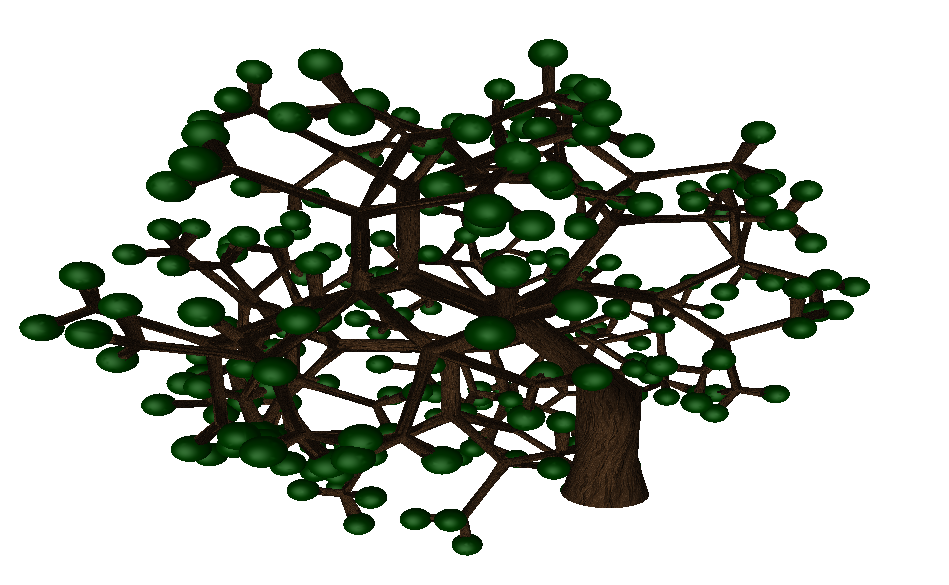
\includegraphics[scale=0.3]{Diagrams/ternarybranching3_a60.png}
		}
		\caption{L-system 2 where the variable `a3' has the value of 60$^\circ$. } \label{extreme example angle}
	}
\end{figure}
\FloatBarrier

\noindent
The previous examples have tested the capabilities of the parametric L-system without having the results simulated. The advantage of having the simulator and interpreter separate to the L-system rewriter is the simulator and interpreter can choose to ignore specific parameters. For instance, if the physical properties of a plant is provided by the L-system, the simulator can easily be turned off, resulting in a static plant. Without running the simulator the plant will become less resource-intensive to render as it is not being continuously updated. The next examples show that changing the physical properties of the plant can change how it responds when the simulator is turned on. Each screenshot is taken after five seconds of the simulator running; this allows the branches' movement to settle into their resting position.

In figure \ref{constant spring} below, the spring constant `scstart' is decresed from 200 to 50.  However, the spring constant modifier `scmod' is 1.0. The spring constant for each branch is rewritten with the current spring constant multiplied by the spring constant modifier. This gives the relationship similar to how the width is calculated $sc_{i+1} = sc_i * scmod$. If the `scmod' value is 1.0, the spring constant will be a uniform value independant of how many generations there are. Leaving the spring constant the same throughout the tree assumes that thick branches at the base of the tree are as bendy as thin branches at the top of the tree. This is not accurate and will result in large branches bending unrealistically, particularly under extreme forces. Although this kind of behaviour would not be realistic, it highlights the flexibility of the system, if the physical properties are changed within the L-system it will have a direct affect on the resulting model and simulation.

\begin{figure}[htbp]
	{\centering
		\vspace{7px}
		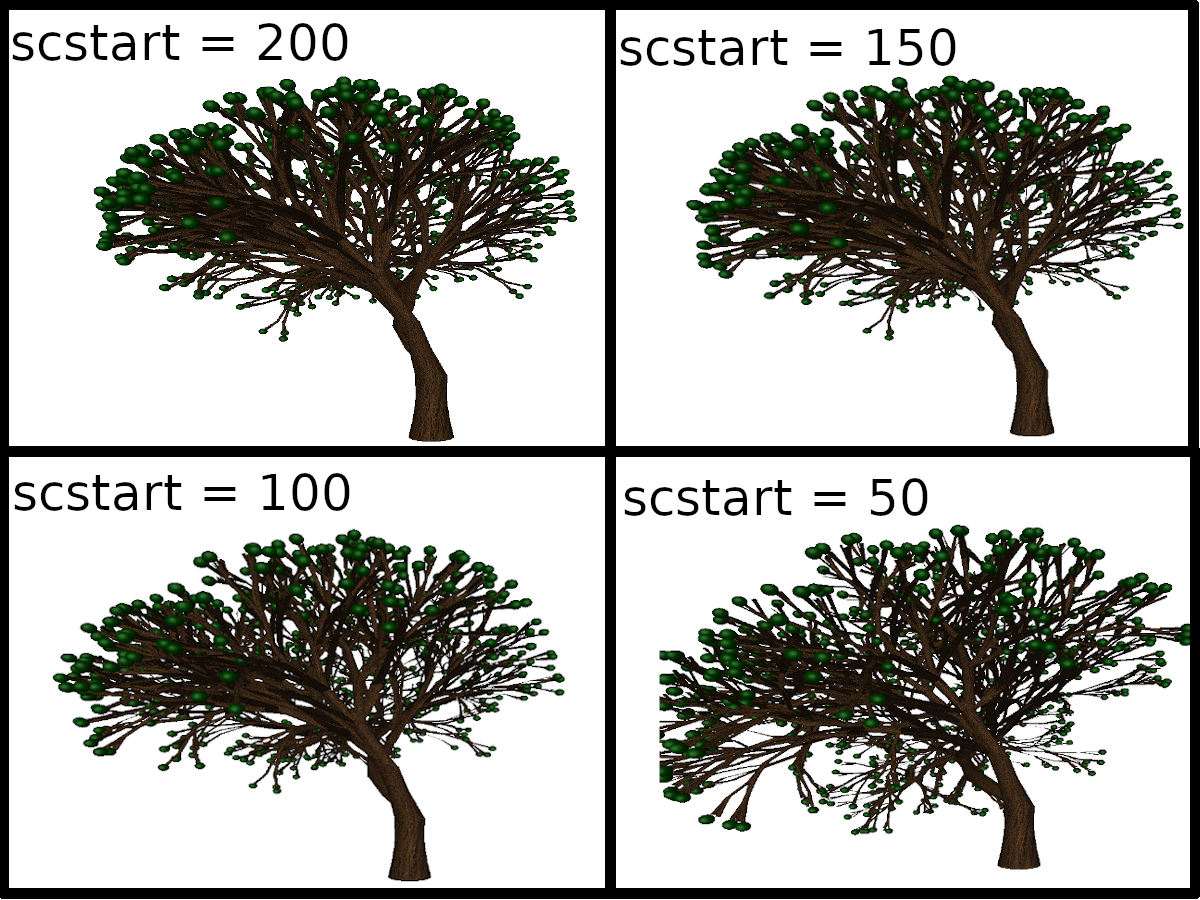
\includegraphics[scale=0.30]{Diagrams/TernaryBranching3_constantSC.png}
		\caption{Examples of L-system 1 when uniformly changing the `scstart' for all branches and leaving `scmod = 1.0'.}\label{constant spring}
	}
\end{figure}
\FloatBarrier

\noindent
In order to create a more realistic simulation where thinner branches bend more than thicker ones, the initial spring constant can be set to 30. The `scmod' value can be increased, resulting in the branches closer to the base being exponentially stiffer. Therefore, branches closer to the top are week and susceptible to smaller forces moving them around. As seen in figure \ref{increasing scmod} below, when the modifier is very high, the larger branches hardly bend at all, whereas, with a lower modifier, the larger branches visibly bend. The graphs in figure \ref{spring constant graphs} show the different ways spring constant and spring constant modifier can be changed to produce different types of branch strengths within the L-system rewriter.

\begin{figure}[htbp]
	{\centering
		\vspace{7px}
		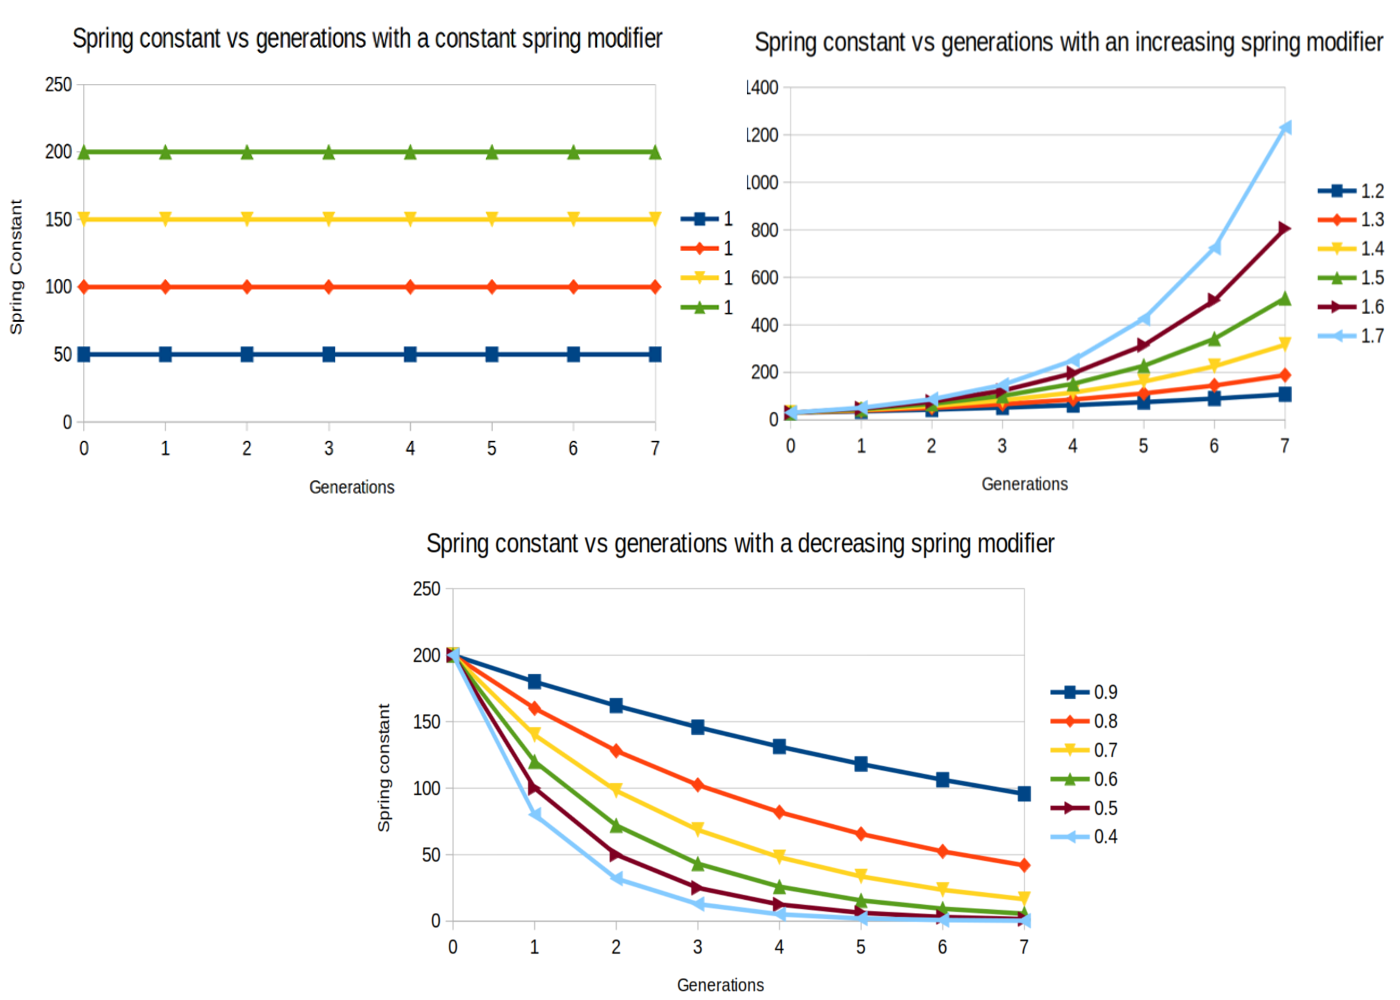
\includegraphics[scale=0.30]{Diagrams/springconstantgraphs.png}
		\caption{Graphs showing the distribution of spring constants dependency on the spring modifier and number of generations.}\label{spring constant graphs}
	}
\end{figure}
\FloatBarrier

\begin{figure}[htbp]
	{\centering
		\vspace{7px}
		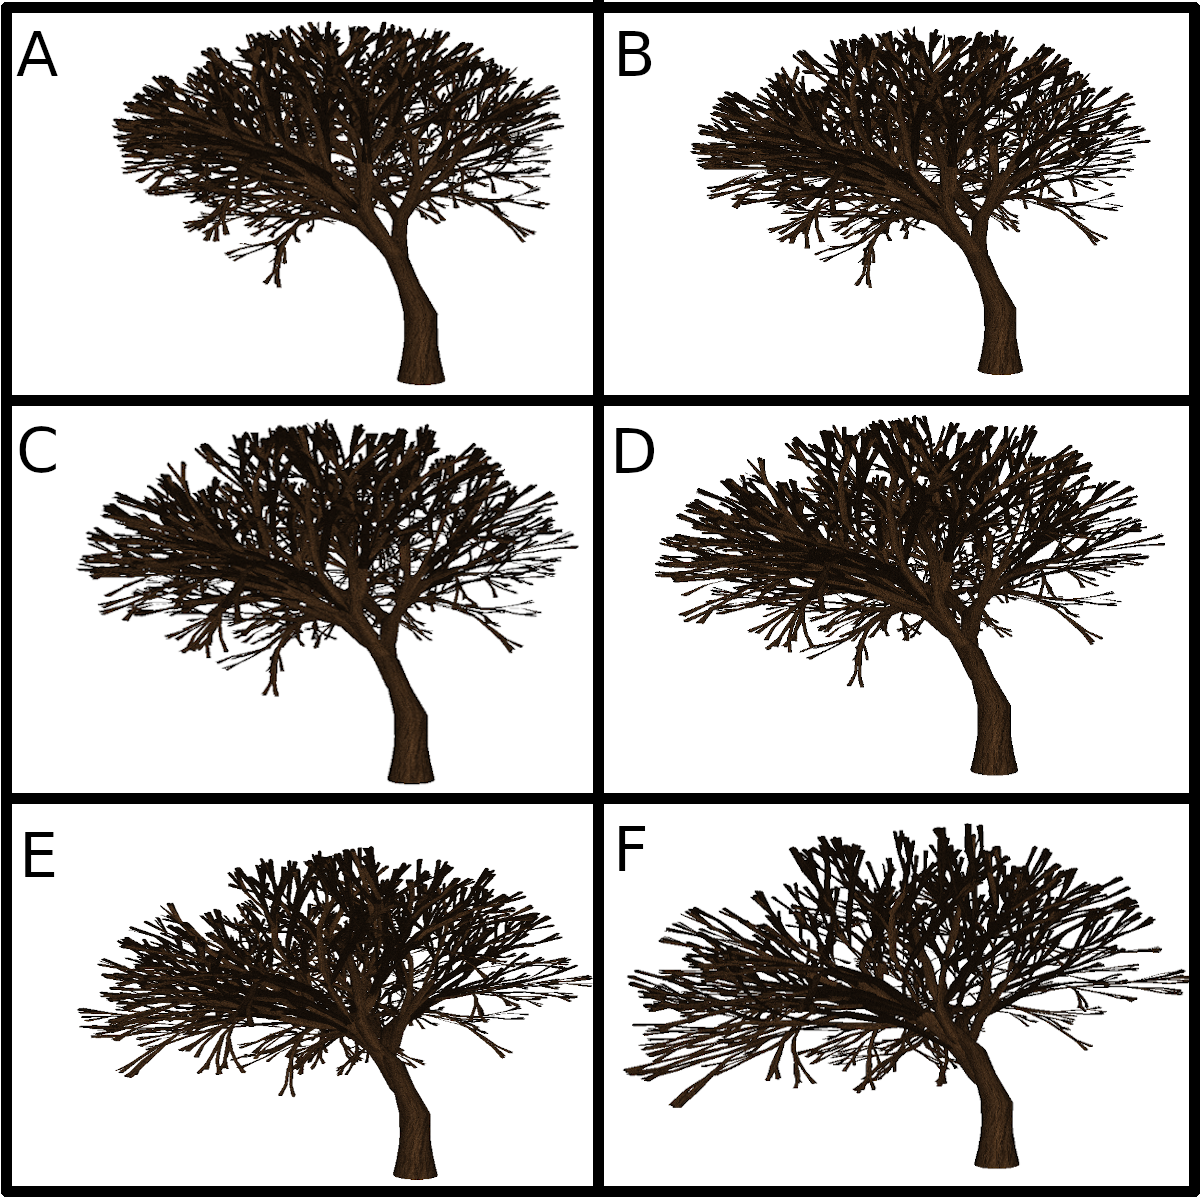
\includegraphics[scale=0.30]{Diagrams/TernaryBranching3_scmod.png}
		\caption{Examples of L-system 3 with gravity applied when changing the spring constant modifier `scmod', when the starting spring constant is set to 30 `scstart = 30'.}\label{increasing scmod}
	}
\end{figure}
\FloatBarrier

\noindent
The L-system \ref{2d L-system physics} below creates the 2D fractal tree that has rendered in three dimensions. It is a 2D tree as it only consists of left and right yaw rotations signified with the `+ and -' symbols without any pitch or roll rotations. In this tree, the rotation `r' is defined as 20$^{\circ}$, the distance `d' is 0.4, and the width `w' is 0.5. The spring constant of the branches is kept at a constant 30.0. This means that all the branches are equally prone to bending. 

\begin{singlespace}
\begin{equation} \label{2d L-system physics}
\begin{aligned}
	&\textrm{\#n = 6;} \\
	&\textrm{\#define r 20; \#define d 0.4; \#define w 0.5;}\\
	&\textrm{\#w : !(w)Z;}\\
	&\textrm{\#p1 : Z : * : F(d, 30.0)[-(r)Z]F(d, 30.0)[+(r)Z]-(r)Z;}\\
	&\textrm{\#p2 : F(s, x) : * : F(s, x)F(s, x);}
\end{aligned}
\end{equation}
\end{singlespace}

\begin{figure}[htbp]
	{\centering
		\vspace{7px}
		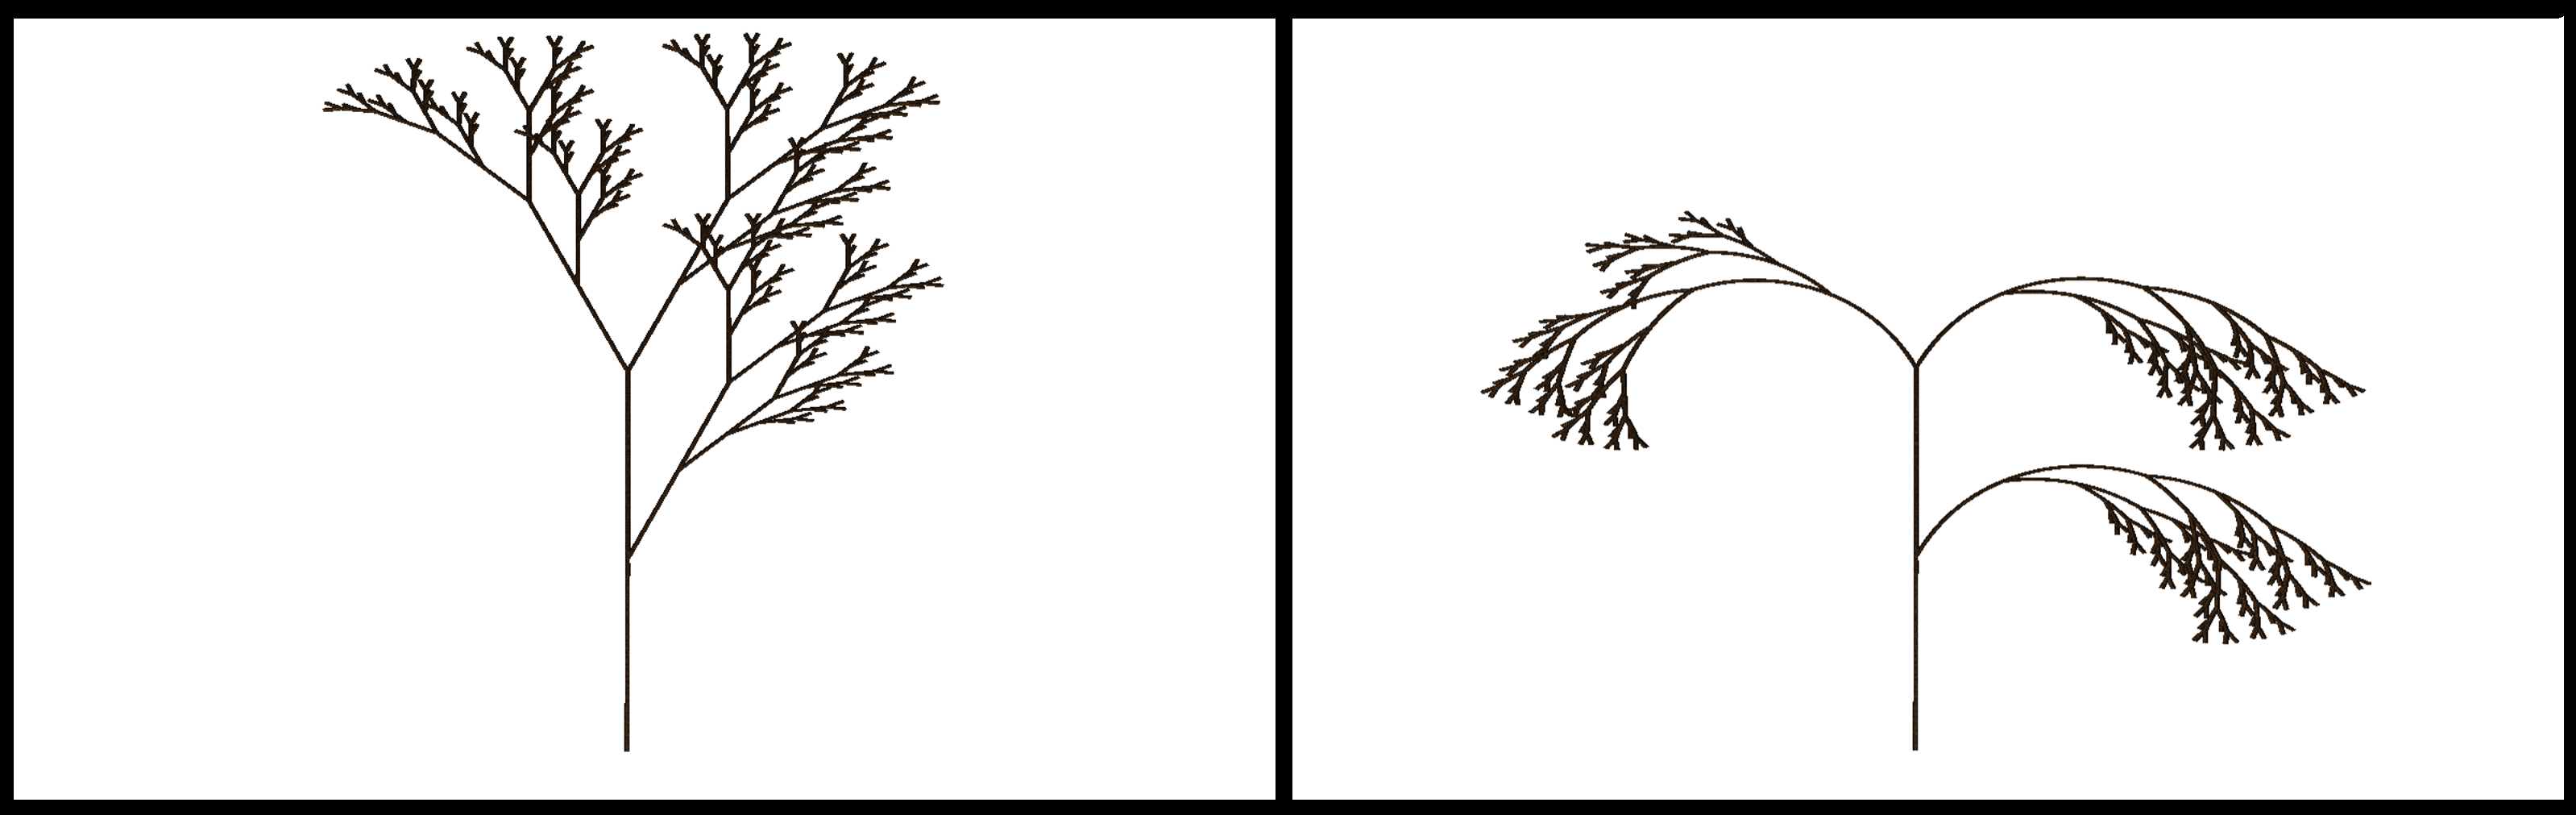
\includegraphics[scale=0.1]{Diagrams/gravityExamples1.png}
		\label{3DAxisFigure} \label{Gravity applied to generated model 1}
		\caption{Examples simulating gravity on a 2D model}
	}
\end{figure}
\FloatBarrier

\noindent
The L-system and figure below produces a structure similar to a pine tree. The tree consists of a a single center branch that has four branches in different directions at several points up the center branch. Although the structure of the plant is very different to the previously mentioned L-systems, providing the parameters for simulation is very similar, and as shown in the figure below can provide a convincing effect when gravity is applied.

\begin{singlespace}
\begin{equation}
\begin{aligned}
	&\textrm{\#n = 5;} \\
	&\textrm{\#object F BRANCH; \#object X SPHERE;}\\
	&\textrm{\#define r 25.7; \#define d 0.5; \#define w 1;}\\
	&\textrm{\#define scstart 30; \#define scmod 1.0;}\\
	&\textrm{\#w : !(1.707)X;}\\
	&\textrm{\#p1 : X : * : F(d, scstart)[!(w)/(r)+(r)X][!(w)-(r)X][!(w)$\land$(r)X][!(w)\&(r)X]!(w)F(d, scstart)X;}\\
	&\textrm{\#p2 : F(s, x) : * : F(s, x * scmod)F(s, x * scmod);}
\end{aligned}
\end{equation}
\end{singlespace}

\begin{figure}[htbp]
	{\centering
		\vspace{7px}
		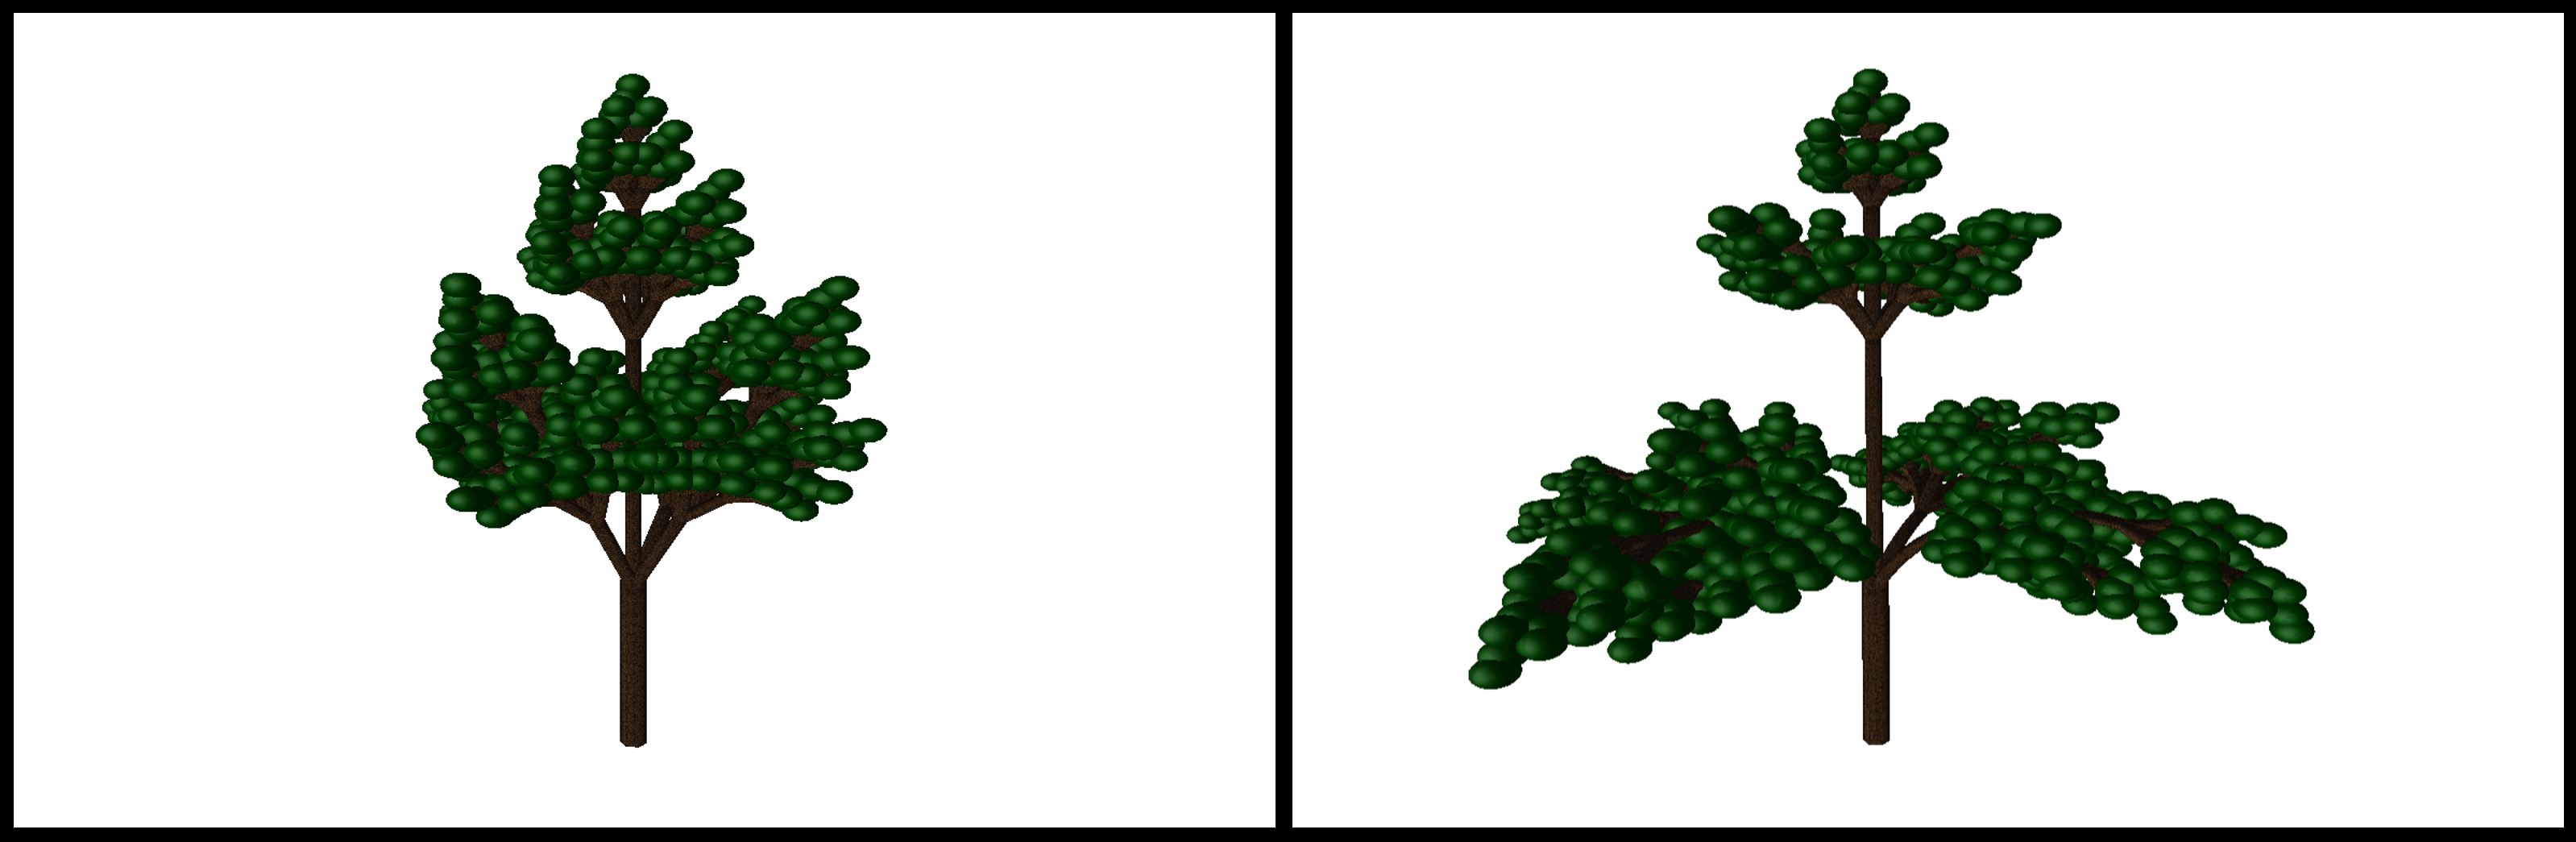
\includegraphics[scale=0.1]{Diagrams/gravityExamples2.png}
		\label{3DAxisFigure} \label{Gravity applied to generated model 1}
		\caption{Simulating gravity on a simple pine tree model.}
	}
\end{figure}
\FloatBarrier

\noindent
In figure \ref{Wind applied to generated model}, the same L-system seen in \ref{Gravity applied to generated model 1} is used, however, the interpreter has been instructed not to render the green spheres at the ends of branches, to see the branching structure better. Instead of gravity the simulator is showing the effect of wind coming from the right hand side of the tree. Each image is a timestep showing an exadurated effect of wind on the plant. In a simulation within a video game or 3D application the wind would be simulated at a lesser extent however you would see a similar movement as well as the russtleing of branches.

\begin{figure}[htbp]
	{\centering
		\vspace{7px}
		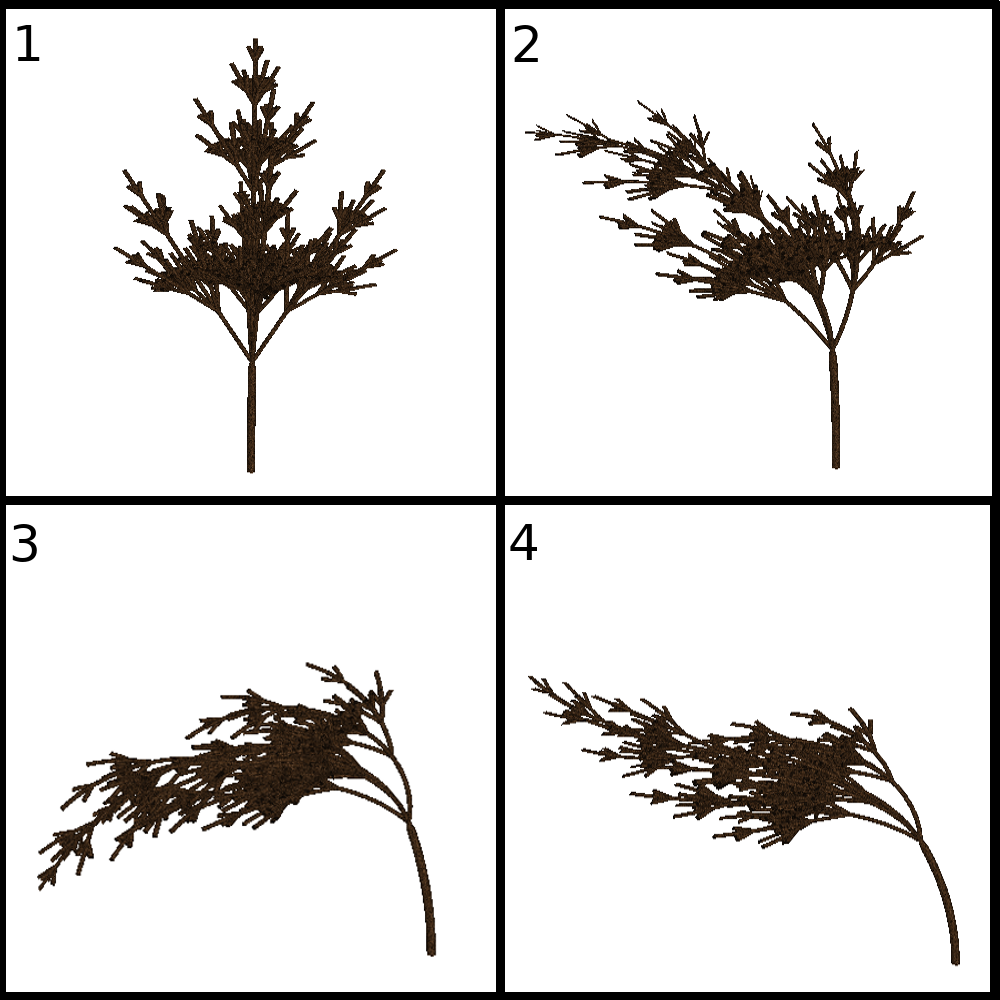
\includegraphics[scale=0.3]{Diagrams/windExample.png}
		\label{3DAxisFigure} \label{Wind applied to generated model}
		\caption{Simulating wind on a simple pine tree model}
	}
\end{figure}
\FloatBarrier

\noindent
The examples and tests in this chapter show that the parametric L-system has the capability of affecting the look of a plant drastically, by changing one or two parameters. Changing these parameters can also affect its behaviour when simulated, either directly with the spring constant or indirectly by changing the length or width of branches. The rewriting mechanism of the L-system makes it well suited for providing the plants' physical information. It is possible to use the rewriting mechanism to change a branches' spring constant depending on the number of times that branch has been rewritten. The trees skeletal structure generated by the turtle graphics interpreter makes it very simple to implement a particle physics system to simulate any generated structure. 


